\subsection{Relation to Bell Inequalities}
  \label{subsec:relation-to-bell-inequalities}

  Bell's theorem~\cite{Bell1964} establishes that no physical theory reproducing the full
  set of quantum mechanical predictions can simultaneously satisfy locality,
  realism understood as outcome determinism conditioned on hidden variables, and statistical independence.
  The empirical violations of Bell inequalities therefore rule out any ontological
  completion of quantum mechanics based on factorizable hidden-variable models.

  The Cosmochrony framework fully accepts Bell's theorem as a fundamental constraint.
  It does not seek to evade or weaken Bell inequalities, nor to restore locality or realism in their classical sense.
  Instead, it identifies the precise ontological assumption that fails within
  Bell-type derivations when applied to admissible projected descriptions.

  \paragraph{Failure of ontological factorisability.}
    Standard Bell-type arguments assume that joint outcome probabilities admit a factorization of the form
    \begin{equation}
      P(a,b|x,y,\lambda) = P(a|x,\lambda)\,P(b|y,\lambda),
    \end{equation}
    where $\lambda$ denotes a complete specification of the underlying ontic state.
    In Cosmochrony, such a decomposition is not available, not because of nonlocal dynamical influences, but because
    admissible projected descriptions are subject to global consistency constraints imposed by the projection
    $\Pi$ (Section~\ref{sec:relational_projection}).

    More precisely, the projection $\Pi$ is generically non-injective: multiple distinct configurations of the
    relational substrate $\chi$ may correspond to the same effective description.
    As a result, admissible projected states are not associated with independent ontic pre-images for their subsystems.
    Entangled systems therefore correspond to equivalence classes of non-separable configurations in $\chi$,
    for which no decomposition into independently specifiable local states exists.
    In this sense, the factorization hypothesis required by Bell-type inequalities is not merely violated,
    but is \emph{ill-defined} within the space of admissible projected descriptions.

  \paragraph{Projection-induced correlations and informational compression.}
    The failure of factorization can be understood as a structural consequence of the
    compressive character of the projection $\Pi$.
    The projection maps a high-dimensional relational configuration space onto a reduced
    effective description by discarding unresolved internal degrees of freedom.
    The corresponding projection fiber $\Pi^{-1}(\chi_{\mathrm{eff}})$ may therefore
    contain a large equivalence class of underlying configurations.

    When this compression is neither negligible nor overwhelming, residual global
    constraints persist across projected subsystems, giving rise to non-factorizable correlations.
    Bell-type violations thus arise naturally in an intermediate regime where the
    effective description is sufficiently coarse-grained to permit subsystem
    separation, yet not so coarse as to erase all global relational structure.
    In contrast, in the limit of extreme coarse-graining, projected descriptions become
    effectively factorized, recovering classical statistical behavior.

    In this view, quantum entanglement corresponds to a critical regime of projection:
    neither a direct reflection of the underlying relational configuration, nor a fully
    classical description obtained by over-compression.

    This critical regime and its interpretation in terms of projective compression are developed independently of Bell
    inequalities in Section~\ref{subsec:entanglement-critical-compression}, where entanglement is shown to arise as a
    structural consequence of non-injective projection rather than as a dynamical or measurement-induced effect.

  \begin{figure}[t]
      \centering
      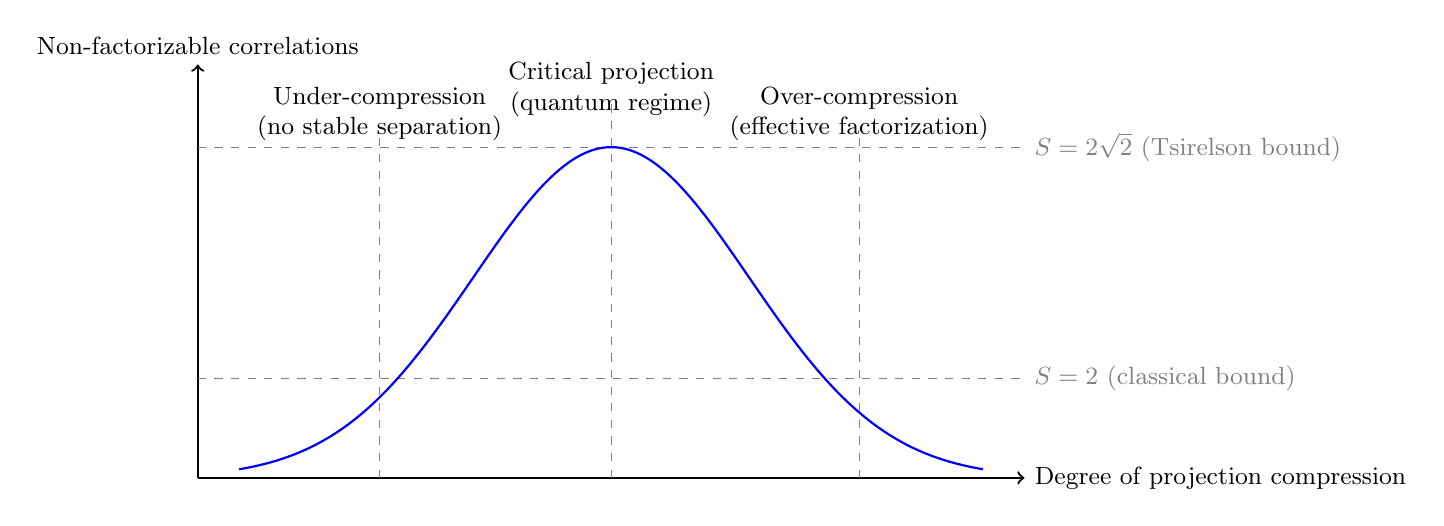
\begin{tikzpicture}[
        scale=1.05,
        axis/.style={->, thick},
        curve/.style={thick, smooth, blue},
        dashedline/.style={dashed, gray},
        label/.style={font=\small}
      ]

% Axes
        \draw[axis] (0,0) -- (10,0) node[right,label] {Degree of projection compression};
        \draw[axis] (0,0) -- (0,5) node[above,label] {Non-factorizable correlations};

% Bell bounds
        \draw[dashedline] (0,1.2) -- (10,1.2)
        node[right,label] {$S=2$ (classical bound)};
        \draw[dashedline] (0,4) -- (10,4)
        node[right,label] {$S=2\sqrt{2}$ (Tsirelson bound)};

% Bell-violation curve
        \draw[curve]
        plot[domain=0.5:9.5,samples=200]
        (\x,{4*exp(-0.18*(\x-5)^2)});

% Regime labels
        \node[label, align=center] at (2.2,4.4)
          {Under-compression\\(no stable separation)};
        \node[label, align=center] at (5,4.7)
          {Critical projection\\(quantum regime)};
        \node[label, align=center] at (8,4.4)
          {Over-compression\\(effective factorization)};

% Vertical guides
        \draw[dashedline] (2.2,0) -- (2.2,4.2);
        \draw[dashedline] (5,0) -- (5,4.6);
        \draw[dashedline] (8,0) -- (8,4.2);

      \end{tikzpicture}
      \caption{Schematic representation of Bell inequality violations as a function of the
      compression induced by the projection $\Pi$.
      Non-factorizable correlations emerge only in an intermediate regime, where the effective
      description is sufficiently coarse-grained to permit subsystem separation, yet retains
      enough global relational structure to prevent factorization.
      In the limit of over-compression, projected descriptions become effectively classical and
      Bell violations disappear.}
      \label{fig:bell-compression-regime}
    \end{figure}

  \paragraph{No hidden variables and no superluminal influence.}
    The absence of ontologically independent subsystems does not introduce hidden variables, local or nonlocal.
    The underlying degrees of freedom are neither accessible nor conditionable, and cannot
    be used to screen correlations or define outcome-determining parameters.
    Accordingly, the violation of Bell inequalities in Cosmochrony does not rely on
    superluminal signalling, retrocausality, or a breakdown of relativistic causal structure.

    Correlations are not mediated, transmitted, or dynamically generated between spatially separated subsystems.
    They reflect global admissibility constraints on projected descriptions, inherited
    from the holistic structure of the underlying configuration space.

  \paragraph{Ontological rather than dynamical nonlocality.}
    Quantum nonlocality in Cosmochrony is therefore ontological rather than dynamical.
    The failure of Bell-type factorizability arises from the structure of admissible
    projected descriptions themselves, not from any nonlocal interaction or exchange of information.
    Bell inequality violations are understood as a manifestation of non-separability
    under projection, rather than as evidence for superluminal causal influences.

    This interpretation preserves the full empirical content of quantum mechanics,
    respects relativistic causality at the operational level, and provides a structural
    explanation for the ubiquity and robustness of entanglement correlations within a
    non-injective relational framework.

  \paragraph{Structural scope of Bell violations.}
    The present analysis establishes the \emph{structural admissibility} of Bell inequality
    violations within Cosmochrony, by identifying the failure of ontological factorisability
    under non-injective projection.
    However, this result does not imply that non-factorizable correlations are uniformly
    realized across all projectable regimes.

    Bell inequalities constrain the logical form of admissible effective descriptions, but
    do not determine the conditions under which such correlations become dynamically or
    operationally accessible.
    The identification of specific regimes in which entanglement is activated, suppressed,
    or extinguished requires additional structural criteria beyond Bell’s theorem itself.

    These regime-dependent aspects of entanglement, including the role of projective
    compression and saturation effects, are addressed independently in
    Section~\ref{subsec:entanglement-critical-compression} and in the numerical investigations
    presented in Appendix~D.
